\documentclass[11pt,fleqn]{article}
%\usepackage{CJK}
\usepackage{latexsym}
\usepackage{color}
\usepackage{graphicx, float}\usepackage{graphicx}
%\usepackage{algorithmicx}
\usepackage{algorithm}
\usepackage{algpseudocode}
%\usepackage[colorlinks]{hyperref}
\usepackage[toc,page]{appendix}
\usepackage{bm}
\setlength{\oddsidemargin}{-0.0in}
\setlength{\evensidemargin}{-0.0in} \setlength{\textwidth}{6.0in}
\setlength{\textheight}{9.0in} \setlength{\topmargin}{-0.2in}

%\setlength{\leftmargin}{0.7in}
\usepackage{amssymb, graphicx, amsmath}  %  fancyheadings,
\usepackage{setspace}
\newcommand\qed{\qquad $\square$}
\newcommand{\nn}{\nonumber}

\def \[{\begin{equation}}
\def \]{\end{equation}}
\def\proof{{\bf Proof:\quad}}
\def \endzm {\quad $\Box$}
\def\dist{\hbox{dist}}


\newcommand{\R}{\mathbb{R}}
%\newtheorem{yinli}{����}[section]
\newcommand{\D}{\displaystyle}
\newcommand{\T}{\textstyle}
\newcommand{\SC}{\scriptstyle}
\newcommand{\FT}{\footnotesize}



%\newtheorem{theorem}{Theorem}[section]
%\renewcommand{\thetheorem}{\arabic{section}.\arabic{theorem}}
\newtheorem{definition}{Definition}
\renewcommand{\thedefinition}{\arabic{section}.\arabic{definition}}
\newtheorem{lemma}{Lemma}[section]
\renewcommand{\thelemma}{\arabic{section}.\arabic{lemma}}
\newtheorem{remark}{Remark}
\renewcommand{\theremark}{\arabic{section}.\arabic{remark}}
\newtheorem{proposition}{Proposition}[section]
\renewcommand{\theproposition}{\arabic{section}.\arabic{proposition}}
\newtheorem{corollary}{Corollary }[section]
\renewcommand{\thecorollary}{\arabic{section}.\arabic{corollary}}
\renewcommand{\theequation}{\arabic{section}.\arabic{equation}}
\renewcommand{\baselinestretch}{1.35}
\newtheorem{exam}{Example}[section]
\renewcommand{\theexam}{\arabic{section}.\arabic{exam}}
\newtheorem{theo}{Theorem}[section]
\renewcommand{\thetheo}{\arabic{section}.\arabic{theo}}
\begin{document}
%\begin{CJK*}{GBK}{song}

\begin{center}

{\LARGE \bf CS391L Machine Learning HW1: Eigendigits }\\

\vskip 25pt
 {Zeyuan Hu, iamzeyuanhu@utexas.edu }\\
\vskip 5pt
{\small EID:zh4378 Fall 2017 }

\end{center}

\begin{spacing}{1.5}
\section{Introduction}

\paragraph{}In this task, we are asked to apply the eigenvector decomposition of covariance for analysis
(also known as \emph{principal components analysis} or PCA) to handwritten image data to recognize
the image identity. The handwritten digit image is described by an $28\times28$ array of brightness values. 
We are given $60000$ exemplars of images with known labels of the digits. Our objective is to 
take a new image and identify the digit in the image. The key element to this task is the similarity metric.
It should be chosen to score the essential variations in the data. This leads to the principal
components anaysis, which identifies the eigenvalues of the covaraince matrix of all the data.

This writeup is organized in the following way: In the following section, I will 
describe the steps to finish the task. Next, I will talk about the experimentation result. 
Lastly, I will give a breif summary of the whole work.

\section{Method}

\paragraph{}In this section, I will talk about how we handle the raw data, how we perform the PCA on the data, and
how we carry out the experiment. 

\subsection{Load the data}

\paragraph{}In file \verb|hw1_report.py|, I first read the data from the disk file called \verb|digits.mat|. There
are $60000$ images with dimension $28 \times 28$ in the training set. The first thing we need
to is to construct the data matrix \verb|data| with $M$ images. I choose first $M$ images
from the training set and I construct matrix \verb|data| with the dimension $784\times M$. Each
column in the \verb|data| matrix is an image. One important step is to convert the datatype of
both our training images and our test images into \verb|float| in Python, which
allows us to keep precision when we do the calculation.

\subsection{Find the eigendigits}

\paragraph{}The first thing we need to do in the PCA is to preprocess the data. Let $\bm{I}_i$ be the 
$784 \times 1$ column vectors with $i = 0, \dots, M-1$. Then we calculate the "average face"
by taking the mean value of each pixel across the whole $M$ images:

$$
\bm{I}_{ave} = \frac{1}{M}\sum_{n=0}^{M-1}\bm{I}_n
$$

Once we get our "average face", we can perform mean normalization by subtracting the "average face"
value of each pixel from the corresponding pixel in the \verb|data| matrix. Now, we are done with
preprocessing of the data. The next thing we do is to calculate the eigenvectors of our covariance
matrix. Covaraince matrix \verb|C| is calculated from $\text{data}^T\times\text{data}$ and we use \verb|numpy.linalg.eig|
function to calculate the eigenvectors of \verb|C|. Once we have the eigenvalues and the corresponding
eigenvectors, we want to sort those two set of values in the descending order. The reason we do this
is that we want to use the eigenvectors with the largest variations as the principal components. We
want to keep \verb|nRedDim| number of eigenvectors and the determination of the exact number of 
\verb|nRedDim| is part of the experiment, which will be described in details in the Results section.
Another step we need to perform before using the eigenvectors is the normalization because we will
construct a new coordinate system with these eigenvectors as basis.

\subsection{Classification on test data}

\paragraph{}Once we are done with the eigenvectors normalization, we are ready to classify the test data.
we use KNN classification algorithm to achieve this goal. Before we apply the
algorithm, we need to transform both the preprocessed test data (i.e., mean normalization) 
and the training data into the coordinate system with our calculated eigenbasis.
Then we can use KNN algorithm to do the classification. KNN algorithm essentially calculates
the euclidean distances between one test sample and all the training examples. Then, the
algorithm selects $K$ (i.e. number of neighbors) shortest distances and assign the label
to the test sample by choosing the mode of the labels of the training examples that
are associated with these $K$ shortest distances.

\section{Results}

\paragraph{}I perform three empirical studies for this task: the first is 
the reconstruction of the test digits; the second is the examination of the relationship
between the classification accuracy and the number of training examples we use; and the
third is the examination of the relationship between the classification accuracy and
the number of eigenvectors we keep.

\subsection{Reconstruct test digits}

\paragraph{}Once we have constructed the eigenspace, the very first thing we want to do is
to check whether the eigenvectors we have calculated are correct or not. This
can be done by projecting the preprocessed test data into our eigenspace and 
then reconstruct them back to its original dimension. We, then, compare the original
the test data with our reconstructed test data and see whether they look similar
(i.e., representing the same digits).

Before ploting the reconstruction of the test digits, we can take a look at what
some eigenvectors may look like. The figure 1 shows the eigenvectors
calculated from training images before mean normalization.

\begin{figure}
\centering
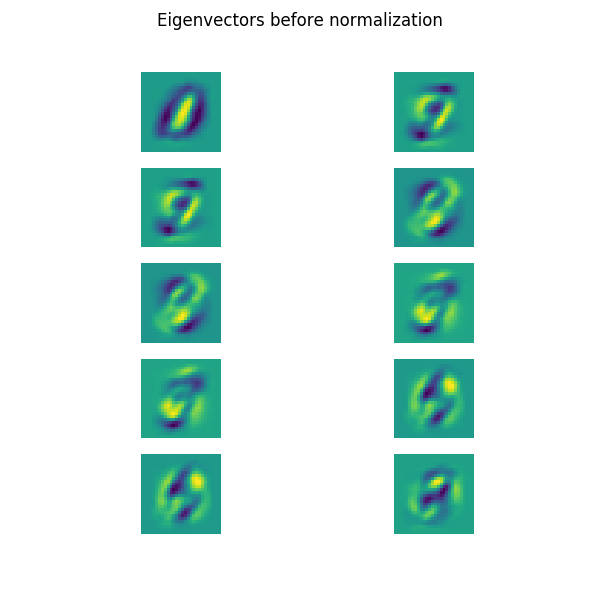
\includegraphics[scale=0.6]{evecs.png} 
\caption{Eigenvectors before normalization}
\end{figure}

The figure 2 shows the result of reconstruction of the first 10 digits
in the test data using the constructed eigenspace.

\begin{figure}
\centering
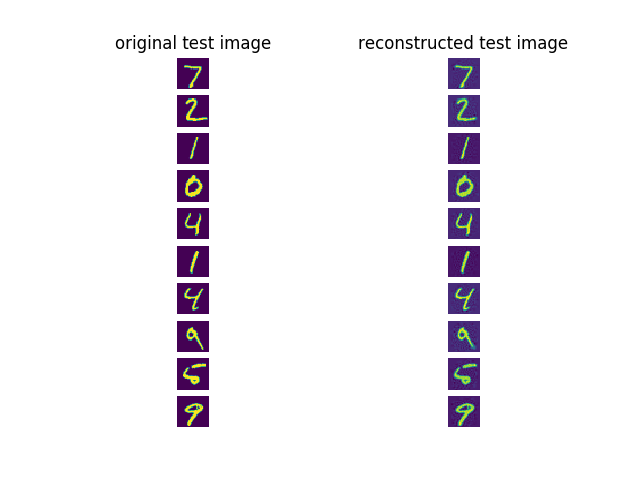
\includegraphics[scale=0.6]{reconstruction_testDigits.png} 
\caption{Reconstruction of the first 10 test digits in the test data}
\end{figure}

\subsection{Classification accuracy vs. number of training examples}

\paragraph{}One thing we want to study about is that how the number of training examples affects
our classification accuracy on the test data. In this experiment, I keep
$20$ eigenvectors and use the training examples ranged from $5$ to $420$. 
$5$ is chosen because our KNN algorithm takes $5$ shortest distances to determine the
label and $420$ is randomly chosen. Figure 3 shows the result of
this experiment. The code for this experiment is wrapped in \verb|numTrain2Accuracy|
function in \verb|hw1_report.py|.

\begin{figure}
\centering
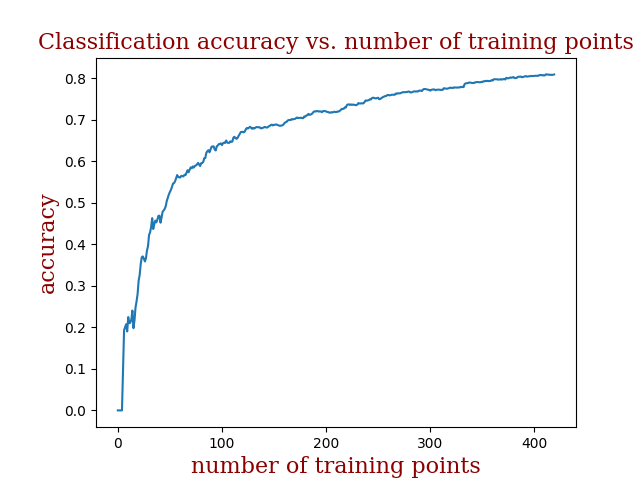
\includegraphics[scale=0.4]{numTrain2Accuracy.png} 
\caption{Classification accuracy vs. the number of training examples}
\end{figure}

\subsection{Classification accuracy vs. the number of eigenvectors we keep}

\paragraph{}In this experiment, I study how the number of eigenvectors impacts our final
classification accuracy in the test data. I use $M = 1000$ training images
to calculate the eigenvectors and I let \verb|nRedDim| go from $1$ to $30$. Figure 4
shows the result of this experiment. The code for this part is listed inside
\verb|nRedDim2Accuracy| function in \verb|hw1_report.py|.

\begin{figure}
\centering
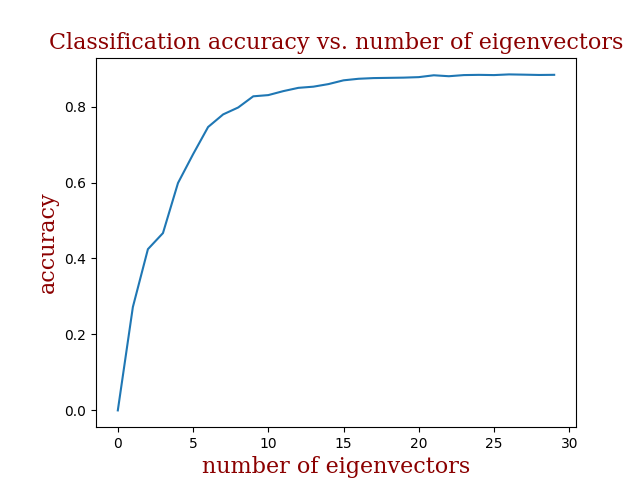
\includegraphics[scale=0.4]{nRedDim2Accuracy.png} 
\caption{Classification accuracy vs. the number of eigenvectors we keep}
\end{figure}

\section{Summary}

\paragraph{}In this task, I apply PCA method to handwritten digits data to perform dimensionality
reduction. Then, I use KNN algorithm to test out how accurate we can identify the digits
in the test data. Afterwards, I explore how the number of training points and the number
of eigenvectors impact our classification performance. The result shows that under the experiment
settings, the classification accuracy is positively correlated with the number of training
examples and the number of eigenvectors. However, we find out there are marginal decrease of 
accuacry gain in both experiments. Specifically, once we get to over $400$ training examples
while keeping the number of eigenvectors fixed, the classification accuracy becomes stable
around $0.85$. Similarly, by keeping the number of training examples fixed, we can get
similar classification performance by keeping at least $30$ eigenvectors.

\end{spacing}

\begin{appendices}

\section{How to run the code}

\paragraph{}To run my code, unzip the \verb|hw1.zip| and put the data file \verb|digits.mat| under the same directory with \verb|hw1_report.py|. Then, you
can run the code with the command \verb|python3 hw1_report.py|. It will output accuracy with different number of training images and different number of eigenvectors. My code is heavily commented and please take a look if there are any type of questions.

\end{appendices}

%\end{CJK*}
\end{document}
